
\section{Experiments}\label{sec:experiments}

\begin{figure}
    \centering
    \begin{subfigure}[t]{0.45\textwidth}
        \centering
        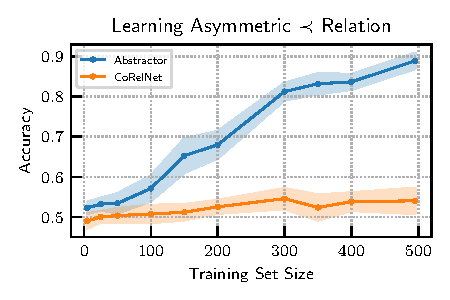
\includegraphics{figures/experiments/pairwise_order_learning_curves.pdf}
        \caption{The Abstractor model follows~\cref{alg:...} with \texttt{num\_layers=1, rel\_dim=4, symbol\_dim=64, proj\_dim=16}. CorelNet uses a dense layer as the embedder $\phi$. The same two-layer MLP is used as the final classification layer in both models. The Abstractor learns the transitive $\prec$ relation and generalizes, whereas CorelNet's learning curve is flat at the baseline accuracy of 0.5.}\label{fig:exp_order_relation}
    \end{subfigure} \hspace{\fill}
    \begin{subfigure}[t]{0.45\textwidth}
        \centering
        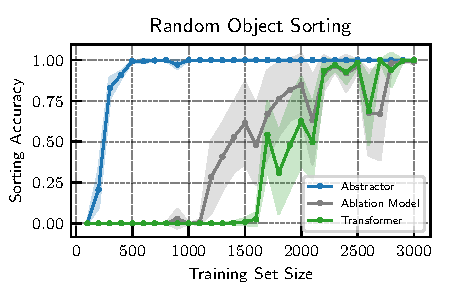
\includegraphics{figures/experiments/random_object_sorting.pdf}
        \caption{...}\label{fig:object_sorting}
    \end{subfigure}

    \bigskip
    \begin{subfigure}[t]{0.45\textwidth}
        \centering
        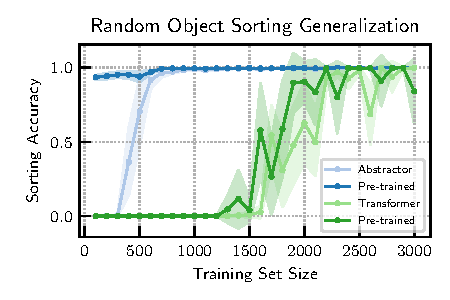
\includegraphics{figures/experiments/random_object_sorting_generalization.pdf}
        \caption{...}\label{fig:object_sorting_generalization}
    \end{subfigure} \hspace{\fill}
    \begin{subfigure}[t]{0.45\textwidth}
        \centering
        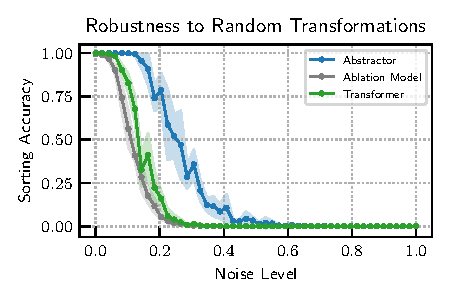
\includegraphics{figures/experiments/multiplicative_robustness.pdf}
        \caption{...}\label{fig:robustness}
    \end{subfigure}
    \caption{Experiments}\label{fig:experiments}
\end{figure}


\subsection{Warm up: Ability to learn asymetric and multi-dimensional relations}
One recent work on relational machine learning is~\cite{corelnet}, where the authors argue for a particular type of inductive bias in relational models and propose CorelNet. The architecture is very simple: given a sequence of objects $(x_1, ..., x_m)$, embed them using an MLP $\phi$, then compute the similarity matrix $A = \left[\langle\phi(x_i), \phi(x_j)\rangle\right]_{ij}$. The final output is an MLP applied to the flattened similarity matrix. They demonstrate that this model can solve a series of simple tasks with high sample-efficiency compared to models like [transformers and ESBN]. However, CorelNet has several significant limitations. One is that it is only able to model symmetric relations---$A$ is symmetric by definition. Another limitation is that it can only model single-dimensional relations---for each pair of objects $(i,j)$, their modeled relation is a single-dimensional scalar $A_{ij}$. The Abstractor is able to model a significantly larger class of relations. In particular, it is able to model asymetric and multi-dimensional relations through the $\text{MultiHeadRelation}$ operation. This is demonstrated by the following simple experiment (as well as the experiments proceeding it).

We generate $N = 32$ ``random objects'' represented by iid Gaussian vectors, $o_i \overset{iid}{\sim} \mathcal{N}(0, I_d) \in \mathbb{R}^d$, and associate an order relation to them $o_1 \prec o_2 \prec \cdots \prec o_N$. We train several different relational models to learn this order relation. Note that $\prec$ is \textit{not symmetric}. Of the $N^2 = 1024$ possible pairs $(o_i, o_j)$, 35\% are held out as a test set and 15\% are held out as a validation set (for early stopping). We evaluate learning curves by training on the remaining 50\% and computing accuracy on the test set. Note that under this set up, we are evaluating the models on pairs they have never seen. Thus, the models will need to generalize based on the transitivity of the $\prec$ relation. We observe that a simple Abstractor model is able to learn the relation while CorelNet cannot.

\subsection{Superior sample-efficiency on relational tasks compared to plain transformers}

\subsection{Modularity and ability to generalize to similar tasks}

\subsection{Robustness and Out-of-Distribution generalization}